\pagebreak
\subsection{Strumenti adottati}
\label{sez:strumenti-adottati}

\subsubsection{Strumenti organizzativi}
\label{sez:strumenti-organizzativi}

\noindent \textbf{\textit{Jira\\}} 

\noindent \textit{Jira} è un \gls{its} che permette la gestione delle attività di progetto in modo \textit{Agile}.\\
I membri del team possono visualizzare le attività assegnate, aggiornare lo stato di avanzamento e comunicare con gli altri membri del team. \\
Durante lo stage è stato utilizzato per la creazione di \textit{epic} e \textit{stories}, la pianificazione delle attività ed il tracciamento dei requisiti.

\begin{figure}[H]
    \label{fig:jira-list-stories}
    \centering
    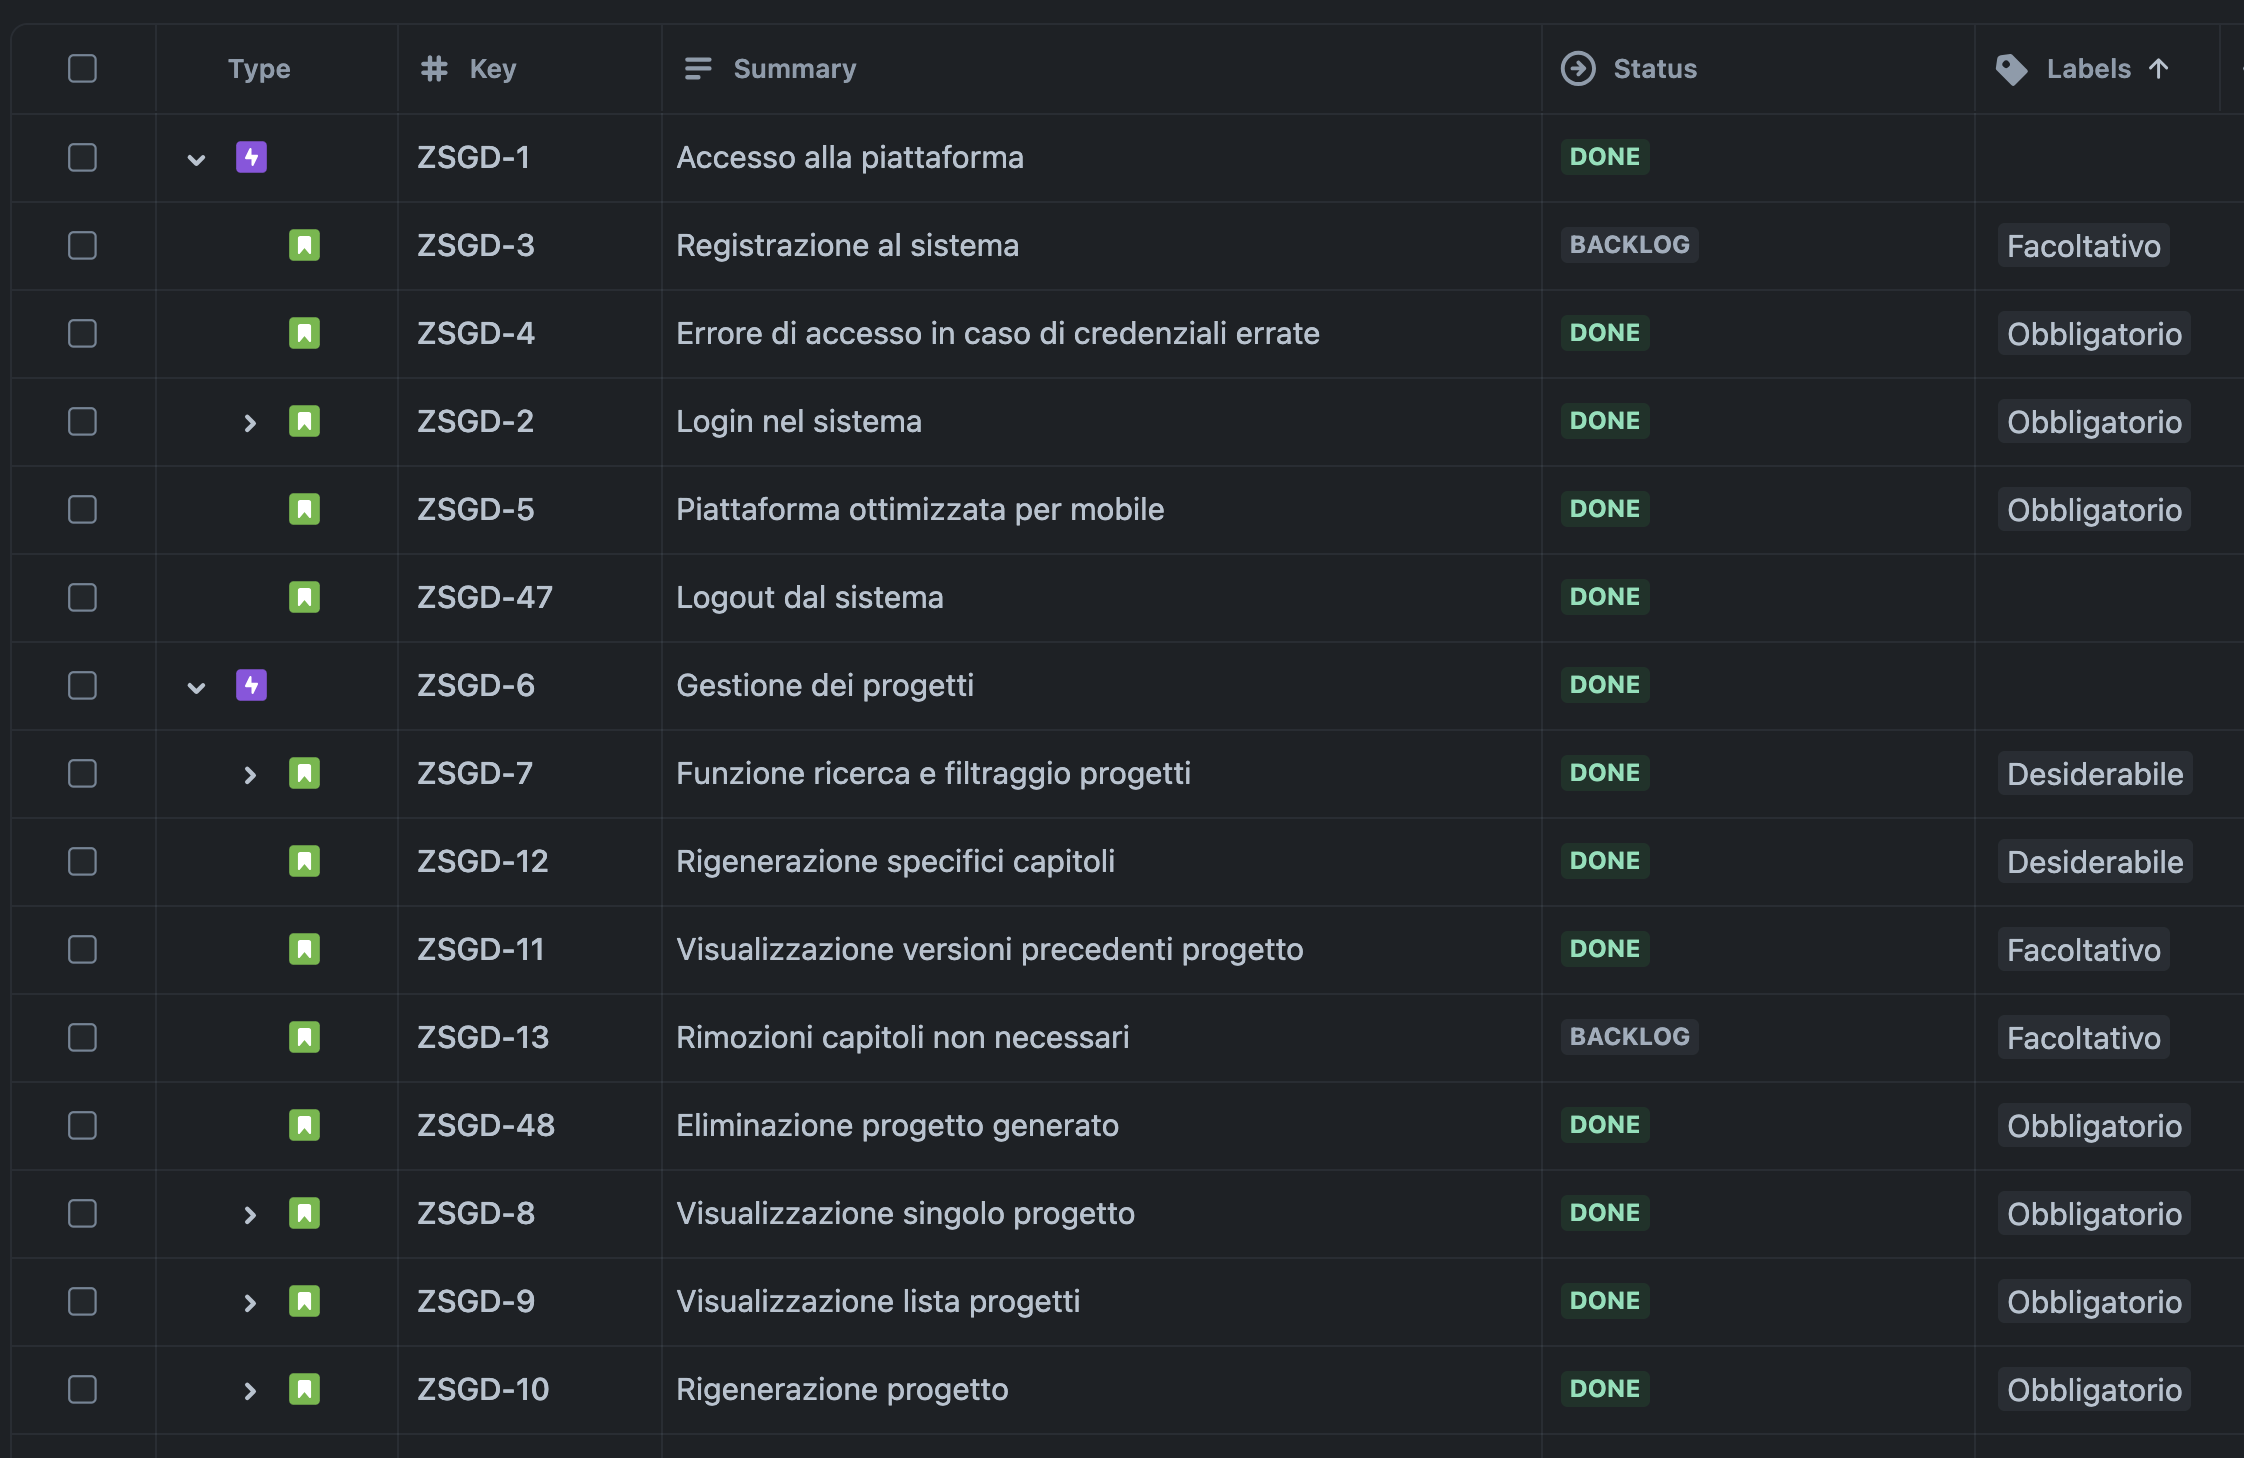
\includegraphics[scale=0.2]{strumenti/jira-list-stories.png}
    \caption{Jira - Lista delle \textit{stories}}
\end{figure}



\noindent \textbf{\textit{Visual Studio Code\\}}

\noindent \textit{Visual Studio Code} è un \gls{ide} sviluppato da Microsoft, che permette la scrittura del codice in diversi linguaggi di programmazione, è stato utilizzato per andare
a sviluppare sia il \gls{frontend} che il \gls{backend} dell'applicazione utilizzando il linguaggio TypeScript.\\

\begin{figure}[H]
    \label{fig:vscode}
    \centering
    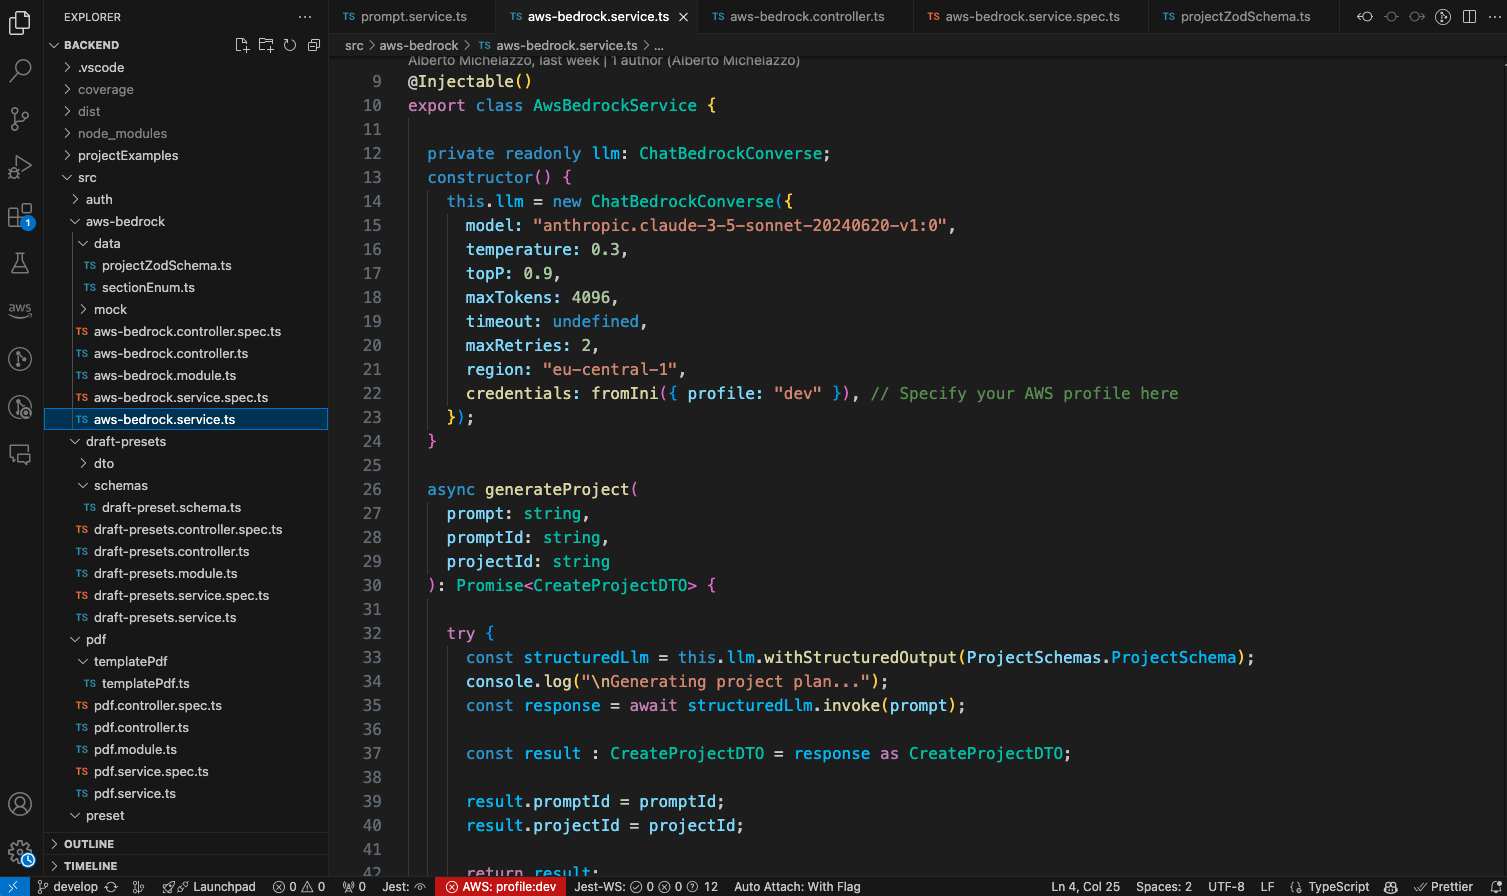
\includegraphics[scale=0.18]{strumenti/vscode.png}
    \caption{VSCode - Interfaccia di sviluppo}
\end{figure}

\pagebreak  
\noindent \textbf{\textit{GitHub\\}}

\noindent \textit{GitHub} è una piattaforma di hosting per progetti software che utilizzano il sistema di controllo di versione \textit{Git}.
Grazie a questa piattaforma è possibile andare a creare \textit{repositories} per il proprio progetto, permettendo la collaborazione tra i membri del team e il tracciamento delle modifiche effettuate. \\
È inoltre possibile andare a a suddividere il progetto in \gls{branch}, per andare a sviluppare le funzionalità tramite cosidetti \textit{feature branch}.
Terminata la codifica di una \textit{feature}, è possibile effettuare una \gls{pr} per andare ad unire il codice sviluppato con il \gls{branch} principale.

\begin{figure}[H]
    \label{fig:github} 
    \centering
    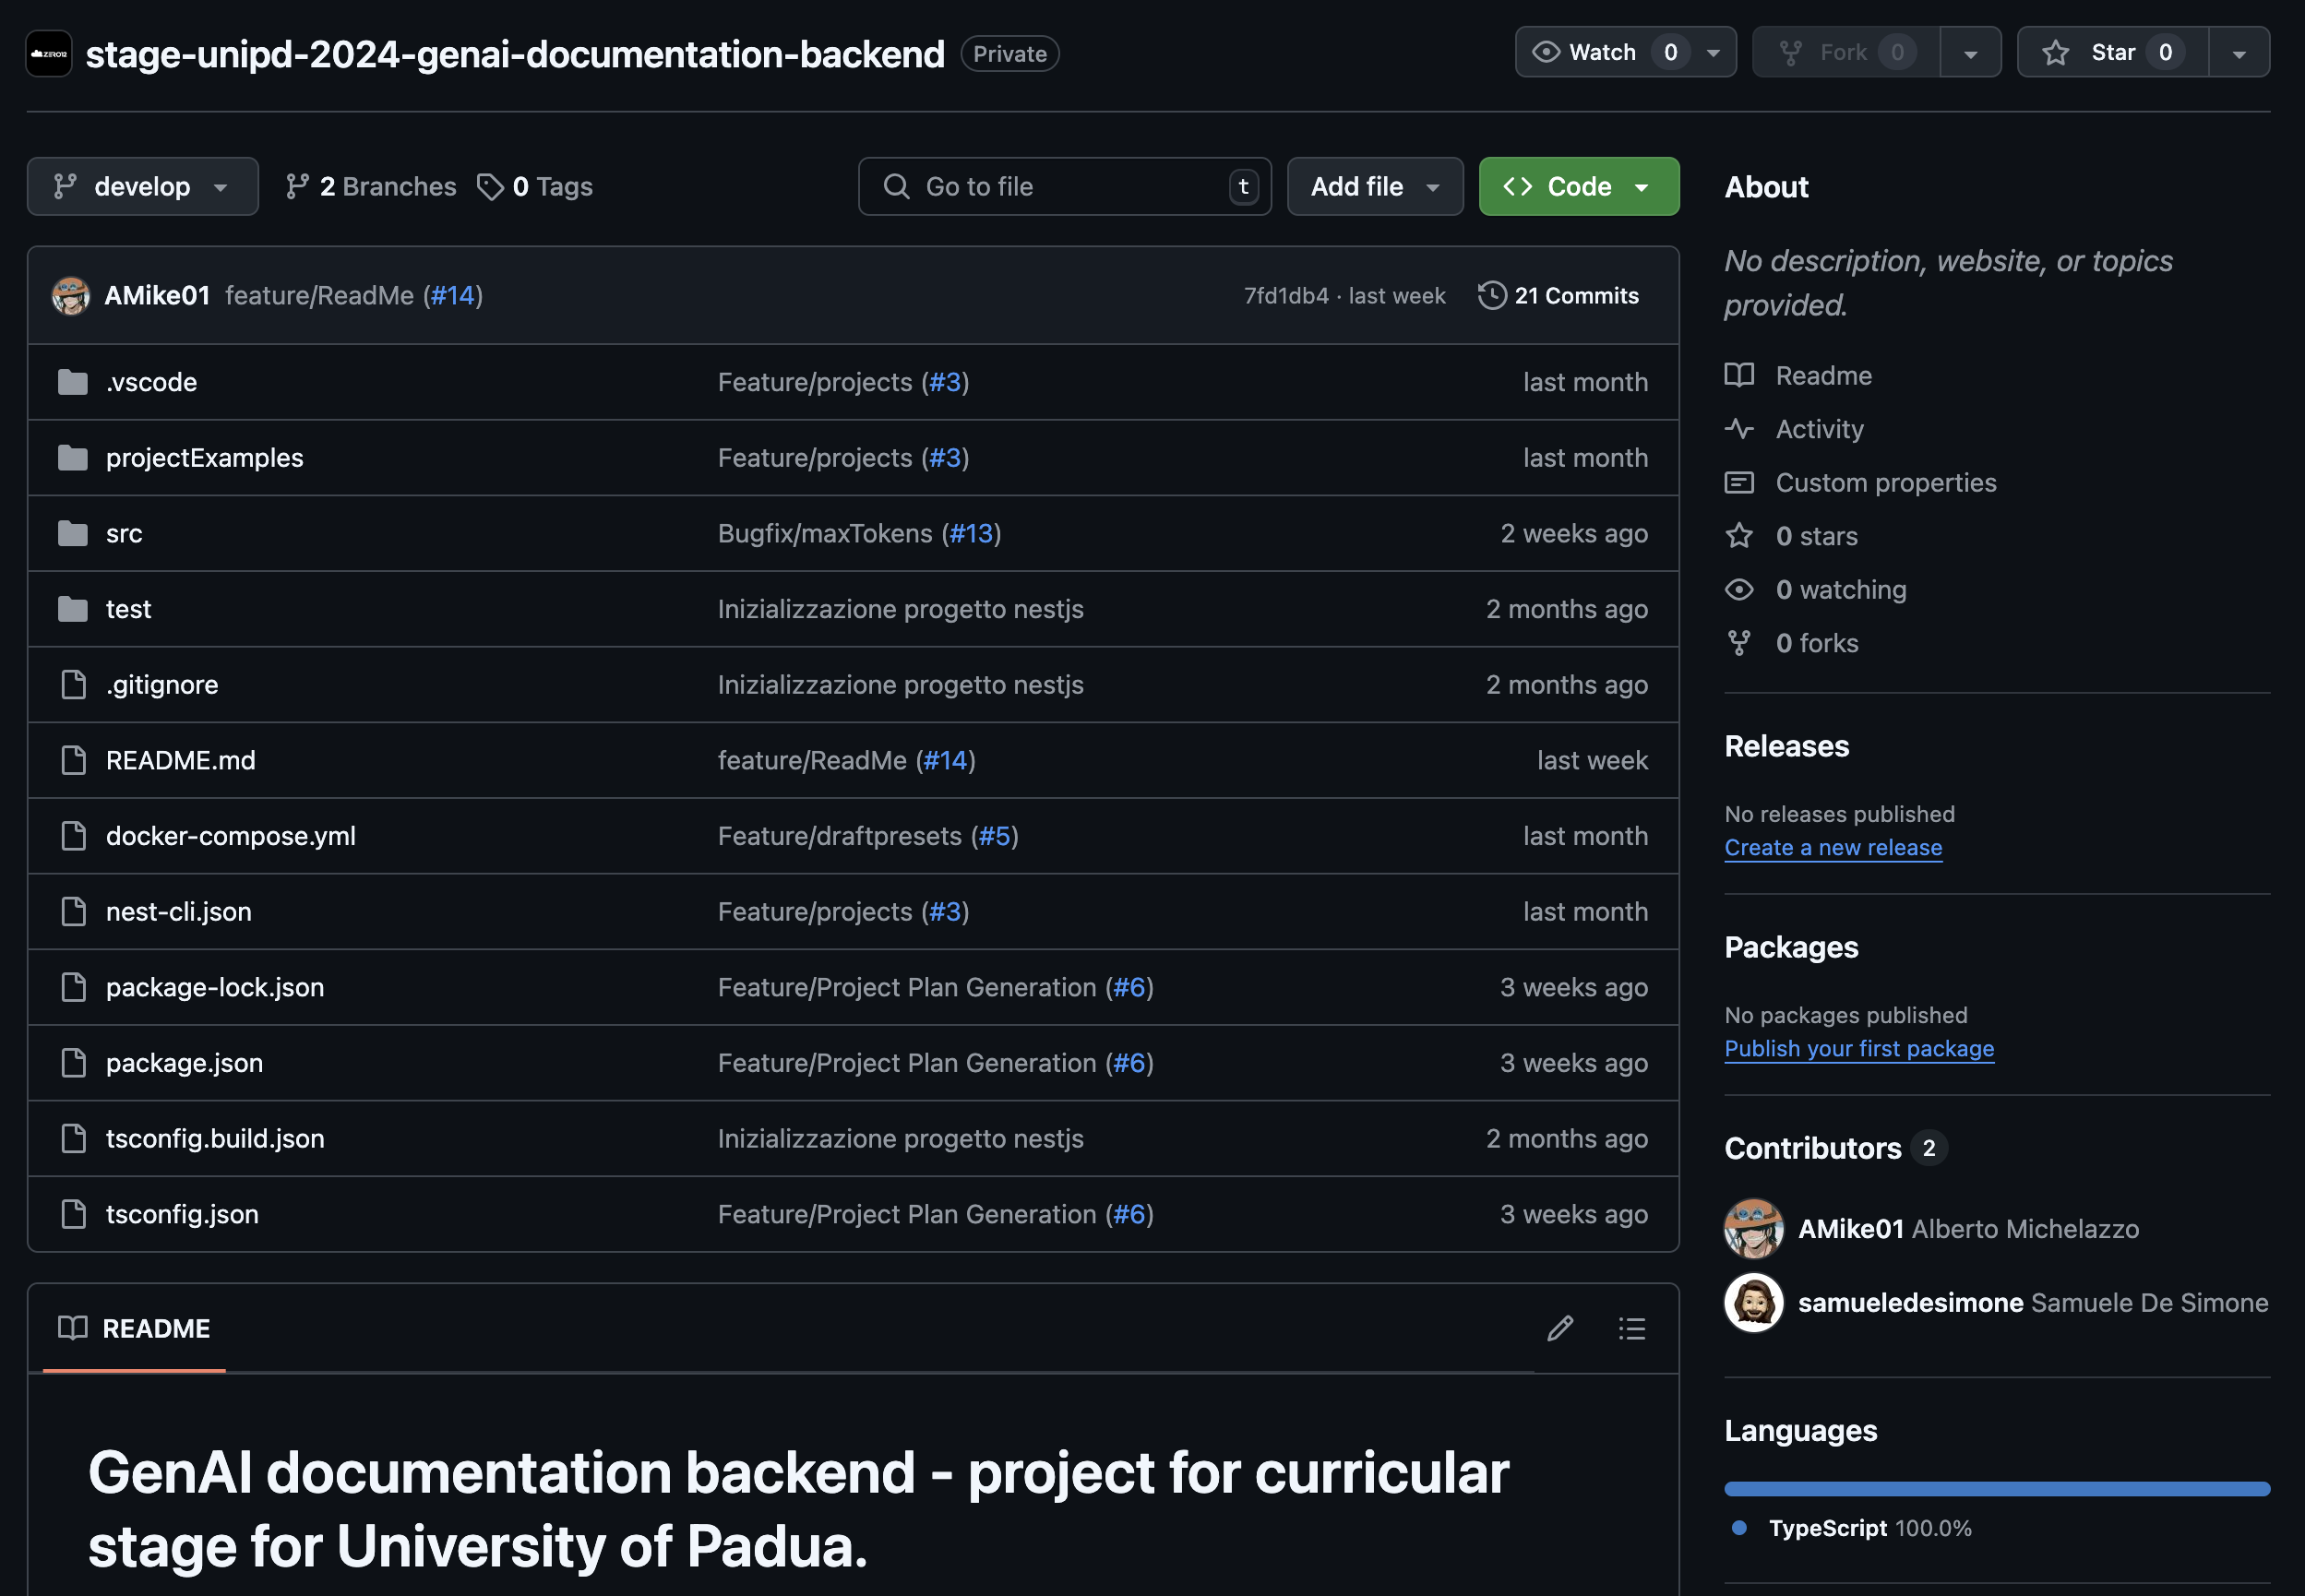
\includegraphics[scale=0.25]{strumenti/github-repo.png}
    \caption{GitHub - Una delle repositories create}
\end{figure}

\pagebreak
\subsubsection{Strumenti di comunicazione}
\label{sez:strumenti-comunicazione}


\noindent \textbf{\textit{Slack\\}}

\noindent \textit{Slack} è un'applicazione di messaggistica istantanea che permette la comunicazione in ambito aziendale. \\
Tramite la creazione di specifici canali è possibile organizzare le conversazioni per progetto, permettendo una comunicazione più efficace tra i membri del team.\\
Nel caso del mio stage è stato creato un canale dedicato al mio progetto, insieme al mio tutor ed ad un'altra figura aziendale, per poter comunicare in modo più diretto e veloce 
in caso di problematiche o dubbi durante lo sviluppo.

\begin{figure}[H]
    \label{fig:slack} 
    \centering
    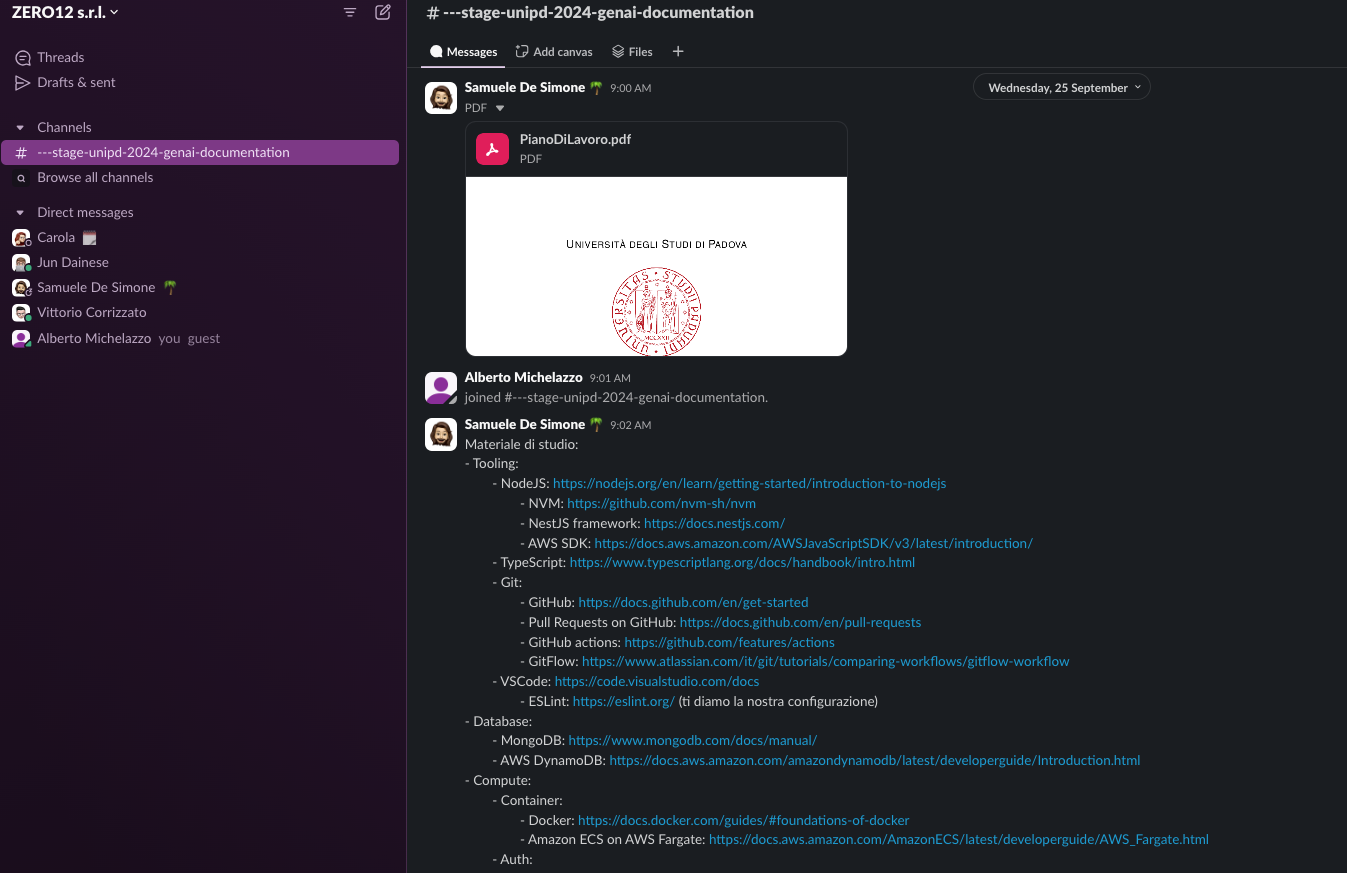
\includegraphics[scale=0.2]{strumenti/slack.png}
    \caption{Slack - Canale dedicato al progetto}
\end{figure}

\noindent \textbf{\textit{Microsoft Teams\\}}

\noindent \textit{Microsoft Teams} è un'applicazione di collaborazione che permette la comunicazione tra i membri del team, la condivisione di file e la gestione di riunioni.\\
Durante il mio stage è stato utilizzato per la gestione delle riunioni settimanali con il tutor aziendale, per discutere lo stato di avanzamento del progetto e per ricevere feedback sul lavoro svolto, quando
non era possibile effettuare un incontro di persona.
